\section{Preliminaries}
\label{sec:preliminaries}

\subsection{Data Model}
Let $L$ be a finite set of labels, $D = \bigcup_i D_i$ be the union of atomic domains $D_i$, and $\epsilon$ be the \kw{NULL} value. We define a \textit{property graph} as $G = (V, E, \lambda, L, T, \vlabel, \elabel, P_v, P_e)$, where
\begin{itemize}
    \item $V$ is a finite set of vertices,
    \item $E$ is a finite set of edges,
    \item $\lambda: E \mapsto V \times V$ connects each edge $e$ with a tuple $(s, t)$ of source and target vertices,
    \item $\vlabel: V \mapsto 2^L$ assigns a set of labels to each vertex,
    \item $\elabel: E \mapsto T$ assigns a type to each edge,
    \item $P_v$ is a set of vertex properties, where $p_v^i: V \mapsto D_i \cup \{\epsilon\}$ is a partial function that assigns a property value in $D_i$ to each vertex. 
    In particular, if a vertex $v$ does not have the property $p_v^i$, $p_v^i(v) = \epsilon$,
    \item $P_e$ is a set of edge properties, where $p_e^j: E \mapsto D_j \cup \{\epsilon\}$ is a partial function that assigns a property value in $D_j$ to each edge. 
    In particular, if an edge $e$ does not have the property $p_e^j$, $p_e^j(e) = \epsilon$.
\end{itemize}

Let $U = \{a_1, a_2, \ldots, a_n\}$ be a finite set of attributes, then $S = (a_1, a_2, \ldots, a_n)$ is called a schema over $U$. 
The attributes of $S$ is denoted as $\attr(R) = U$. The value of each attribute $a \in \attr(S)$ comes from specific domain, denoted as $\Dom(a)$.
Let $\mathcal{J} = 2^{V \times E \times D}$ be the domain of the sets of records, $\mathcal{J}_D = 2^{D}$ be the domain of the sets of records whose attributes are not vertices or edges. 

Given a property graph $G$, a graph schema is such a schema $S$ that $\forall a \in \attr(S)$, $\Dom(a) \subseteq V \cup E \cup D$. 
In other words, each attribute of a graph schema is either a vertex, or an edge, or data from arbitrary domain. 
A relation $R$ over a graph schema $S$ (i.e. $\sch(R) = S$) is called a graph relation. 
For simplicity, we denote $\attr(R)$ in short for $\attr(S)$ with $\sch(R) = S$ to retrieve the attributes of a graph relation $R$. 
We write $R.a$ to access a given attribute $a$ in the relation $R$. 

Given a graph relation $R$, if $a \in \attr(R) \subseteq V \cup E$, we can further access the property $p$ on the vertex/edge attribute via $p(R.a)$ (or $p(a)$ if the relation $R$ is clear in the context). 
Particularly, we use $\id$ and $\lab$/$\type$ to denote the built-in properties of the globally unique identifier and label/type of a vertex/edge. 
To clarify ambiguity, the term ``attribute'' always refers to the attribute of a relation, while the term ``property'' always refers to the property of a graph element in this article.


\subsection{Graph Relational Algebra}

In this paper, we extend the graph relational algebra for openCypher proposed in \cite{}.
The graph relational algebra utilizes graph relations as its outputs, and consists of operators for graph relations, such as selection ($\sigma$), projection ($\pi$), natural join ($\Join$), left-outer join ($\leftouterjoin$), get-vertices ($\bigcirc$), expand ($\updownarrow^{(w:L)}_{(v)}[e](r)$), and unwind ($\omega$).
Graph relations default apply the \emph{bag} semantics, and assume no order for the relation unless an explicit \emph{sorting} operator is applied.
In this subsection, these operators in graph relational algebra are first introduced with examples.


\subsubsection{Source}
The source operator gets vertices from a graph according to the constraints specified on the labels of the vertices.

\begin{definition}
    The source operator $\bigcirc_{(v:l_1, \cdots, l_k)}$ gets a set of vertices from the graph.
    Each obtained vertex should contain the specified labels $l_1, \cdots, l_k$.
\end{definition}

\begin{figure*}
    \centering
    \begin{subfigure}[b]{0.4\linewidth}
        \centering
        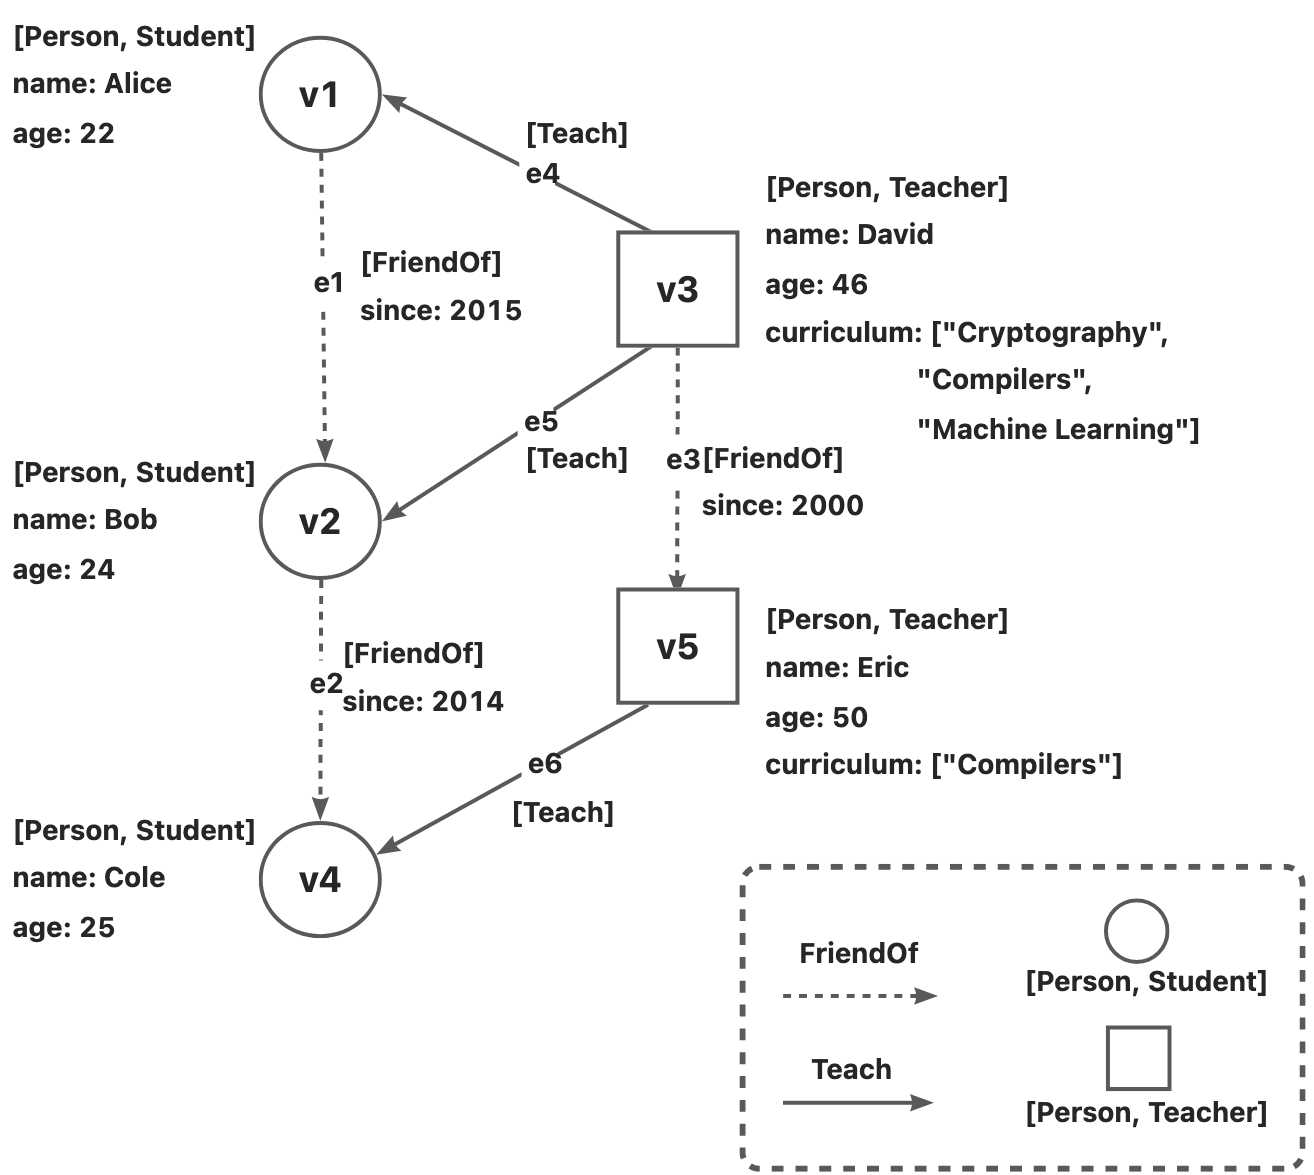
\includegraphics[width=\linewidth]{./figures/example-graph.png}
        \caption{Example Graph.}
        \label{fig:example-graph}
    \end{subfigure}
    \begin{subfigure}[b]{0.4\linewidth}
        \centering
        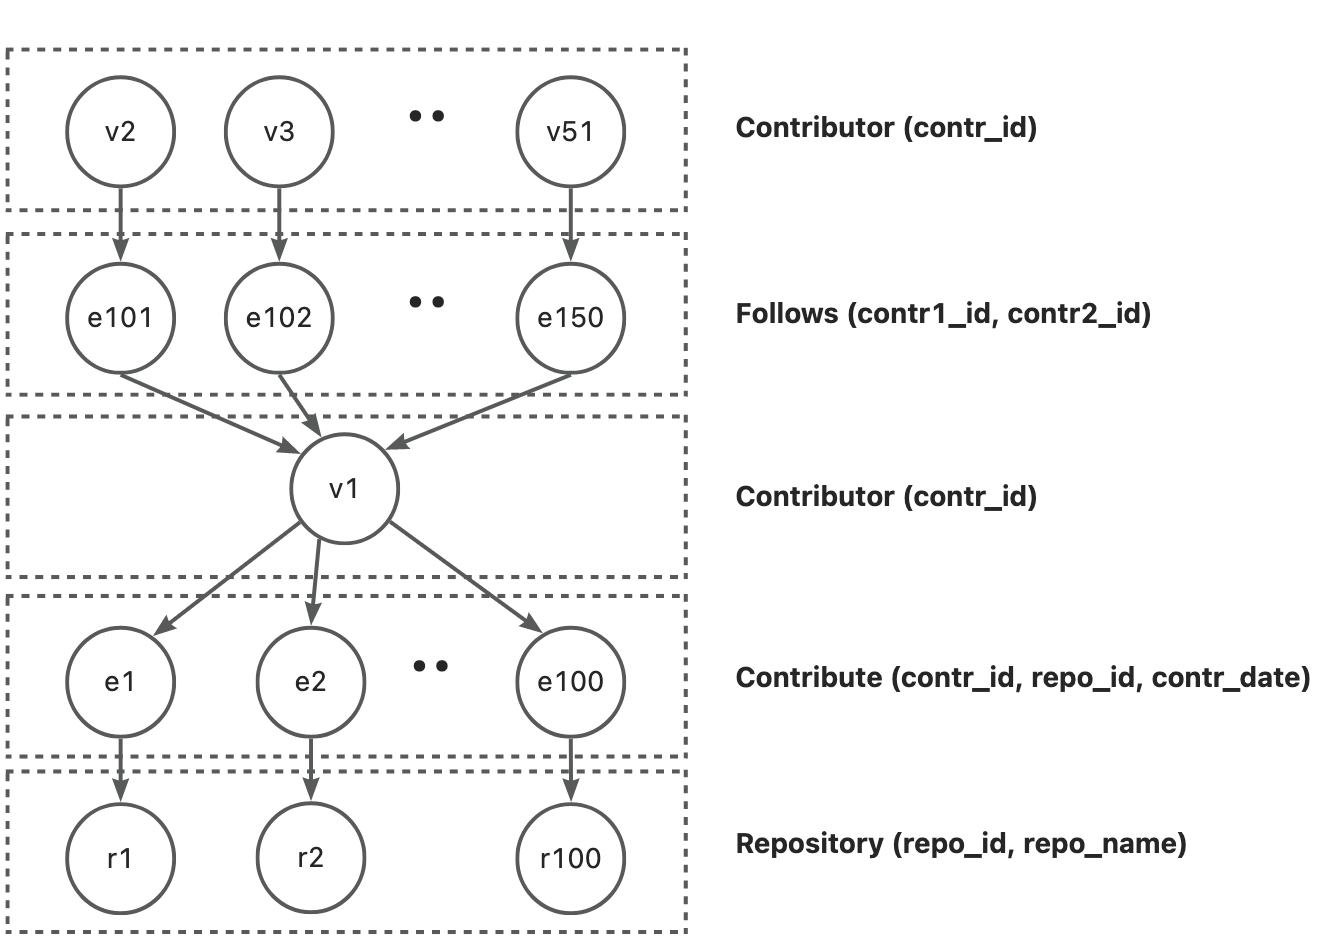
\includegraphics[width=\linewidth]{./figures/intro-order-case-2.png}
        \caption{Formal Definition of Example Graph.}
        \label{fig:example-graph-def}
    \end{subfigure}
    \caption{Definition of an example graph.}
    \label{fig:example-graph-full}
\end{figure*}

\begin{example}
    Suppose property graph $G = (V, E, \lambda, L, T, \mathcal{L}, \mathcal{T}, P_v, P_e)$ represents the relationships among persons.
    The property graph is shown in Fig.~\ref{fig:example-graph}.

    In detail, $V = \{v_1, v_2, v_3, \cdots\}$, $E = \{e_1, e_2, e_3, \cdots\}$, $\lambda = \{e_1 \rightarrow (v_1, v_2), e_2 \rightarrow (v_3, v_1), e_3 \rightarrow (v_3, v_2), \cdots\}$, $\mathcal{L} = \{v_1 \rightarrow \{Person, Student\}, v_2 \rightarrow \{Person, Student\}, v_3 = \rightarrow \{Person, Teacher\}, \cdots\}$, $\mathcal{T} = \{e_1 \rightarrow Friend, e_2 \rightarrow Teaching, e_3 \rightarrow Teaching, \cdots\}$, $p_{v_1}^{\text{name}} = \text{"Alice"}$, $p_{v_1}^{\text{age}} = \text{22}$, $p_{v_2}^{\text{name}} = \text{"Bob"}$, $p_{v_2}^{\text{age}} = \text{24}$, $p_{v_3}^{\text{name}} = \text{"David"}$, $p_{v_3}^{\text{age}} = \text{46}$, $p_{v_3}^{\text{curriculum}} = [\text{"Cryptography"}$, $\text{"Compilers"}$, $\text{"Machine Learning"}]$, $p_{e_1}^{\text{since}} = \text{2015}$. 

    Then, to find all the persons with label \text{Student}, the corresponding expressions is:
    \begin{equation*}
        \bigcirc_{(v_1\text{:Person})}.
    \end{equation*}
\end{example}


\subsubsection{Selection}

The selection operator is used to filter out the records that do not satisfy the specified constraints.
The formal definition of the selection operator is as follows.

\begin{definition}
    The selection operator is a mapping $\sigma_d : \mathcal{J} \rightarrow \mathcal{J}$, where $d$ represents the constraints the resultant records should satisfy.
\end{definition}

\begin{example}
    To find all the students whose name is ``Bob'', the following expression can be used:
    \begin{equation*}
        \sigma_{v_1.\text{name} = ``Bob''}\bigcirc_{(v_1\text{:Student})}.
    \end{equation*}
\end{example}

\subsubsection{Projection}
The projection operator bridges the gap between graphs and tables, which make it possible to combine graph and relational queries.
Its formal definition is as follows.

\begin{definition}
    The projection operator is a mapping $\pi : \mathcal{J} \rightarrow \mathcal{J}$, which maps vertices and edges to a subset of them or their properties, and maps other attributes to a subset of them.
\end{definition}

Please note that if the resultant records of a projection operator cannot contain any vertex or edge, then it is called a flatten projection operator $\hat{\pi} : \mathcal{J} \rightarrow \mathcal{J}_D$.
A flatten projection operator can convert a property graph to a relational table.

\begin{example}
    Suppose we are going to get a relational table of persons, and the schema of the table is (name, age).
    Then, the following expression can achieve the goal.
    \begin{equation*}
        \pi_{v.name, v.age}(\bigcirc_{(v:Person)}).
    \end{equation*}
\end{example}

\subsubsection{Expand}

The expand operator gets the edges adjacent to the given vertices.
Based on the direction of the expansion, the expand operator can be categorized into three types, i.e., expand-out ($\uparrow$), expand-in ($\downarrow$), and expand-both ($\updownarrow$).
For simplicity, the definition of the expand-both operator is given as follows, and those of expand-out and expand-in are similar.

\begin{definition}
    The expand-both operator is a mapping $\updownarrow_{(v)}^{(w:L)}[e] : \mathcal{J} \rightarrow \mathcal{J}$.
    For each record $c$ containing vertex $v$ and each edge $e$ satisfying $\lambda(e) = (v, w)$ (or $\lambda(e) = (w, v)$), a new record is created by appending ($e$, $w$) to $c$.
\end{definition}
 
\begin{example}
    To get all the ``Teaching''' relationships between students and teachers, the following expression can be used:
    \begin{equation*}
        \downarrow_{(v)}^{(v_t\text{:Teacher})}[\text{:Teaching}]\bigcirc_{(v\text{:Student})}.
    \end{equation*}
\end{example}

\subsubsection{Join}

The join operator can join two relational tables or join two property graphs.
Similar to that in relational algebra, the join operator in graph relational algebra also has many types, such as natural join ($\Join$), left-outer join, and right-outer join.
For simplicity, the definition of natural join is proposed, and those of other types of joins is similar.

\begin{definition}
    The natural join operator $\Join : \mathcal{J} \times \mathcal{J} \rightarrow \mathcal{J}$ combines two relations if they have the same values on common attributes.
\end{definition}

The natural join operator can be expressed as follows:
\begin{equation*}
    \begin{split}
        & R \Join P = \sigma_{R.a_1 = P.a_1 \land \cdots \land R.a_k = P.a_k}(R \times P), \\
        & \hspace{2em} \text{where } \text{attr(sch($R$))} \cap \text{attr(sch($P$))} = \{a_1, \cdots, a_k\}
    \end{split}
\end{equation*}

\begin{example}
    To obtain the names of the teachers who teach the common friends of Alice and Bob, the following expression can be used:
    \begin{equation*}
        \footnotesize
        \begin{split}
            & \pi_{v_3\text{.name}}( \\
            & \hspace{1em} (\downarrow_{(v_c)}^{(v_3\text{:Person})}[\text{:Teaching}]\updownarrow_{(v_1)}^{(v_c\text{:Person})}[\text{:Friend}]\sigma_{v_1\text{.name=``Alice''}}(\bigcirc_{(v_1\text{:Person})})) \\
            & \hspace{1em} \Join (\updownarrow_{(v_2)}^{(v_c\text{:Person})}[\text{:Friend}]\sigma_{v_2\text{.name=``Bob''}}(\bigcirc_{(v_2\text{:Person})}))\\ 
            & )
        \end{split}
    \end{equation*}
\end{example}

\subsubsection{Aggregation}
The aggregation operator groups the records according to the values of the specified attributes, and output new records that may contain aggregated values.
The aggregation operator is denoted by $\gamma_{c_1, \cdots, c_i}^{o_1, \cdots, o_j}$.
Specifically, the records are grouped according to attributes $c_1, \cdots, c_i \in V \cup E \cup D$, and $o_1, \cdots, o_j$ are the outputed new attributes.

\begin{example}
    To count the number of students teached by David, the following expression can be used:
    \begin{equation*}
        \downarrow_{(v_1)}^{(v_s:Student)}[\text{:Teaching}]\sigma_{v_1\text{.name=``David''}}(\bigcirc_{(v_1:Person)})
    \end{equation*}
\end{example}

\subsubsection{Sorting and Top}

The sort operator $\tau_{* a_1, \cdots, * a_n}$ is used to sort the input graph relation according to attributes $a_1, \cdots, a_n \in D$.
Specifically, `*' can be $\uparrow$ or $\downarrow$, representing sorting the records ascendingly or descendingly, respectively.
The results of the sort operator are put in an ordered list rather than a bag.

The top operator $\lambda_k^s$ skips the first $s$ records in the input list, and return the next $k$ records as the outputs.
Since the \emph{bag} semantics are applied in graph relations, the records are unsorted by default and the top operator is meaningless in such bags. 
Therefore, the sort operator is usually applied before the top operator is used.

\begin{example}
    To obtain the most aged five teachers, the utilized expression can be as follows:
    \begin{equation*}
        \lambda_{0}^{5}\tau_{\downarrow \text{age}}(\bigcirc_{(v_1\text{:Teacher})})
    \end{equation*}
\end{example}


\subsubsection{Unwind}

Given a graph relation $R$, suppose attribute $xs \in \text{attr}(\text{sch}(R))$ is a list.
Then, for each record $r$ in $R$, the unwind operator appends each value in $r.x$ to $r$ respectively and removes attribute $xs$ from $r$ to generate new records.
The formal definition of the unwind operator is as follows.

\begin{definition}
    Given graph relation $R$ with $\text{sch}(R) = (a_1, \cdots, a_n)$.
    Without loss of generality, suppose the value of attribute $a_1$ is of list type.
    Then, we have $\text{sch}(\omega_{a_1 \rightarrow a_s}(R)) = (a_2, \cdots, a_n, a_s)$.
    For each record $(val_1, \cdots, val_n) \in R$ with $val_1 = [l_1, \cdots, l_k]$,  $k$ new records are generated, where $r'_j = (val_2, \cdots, val_n, l_j)$, $j \in \{1, \cdots, k\}$.
\end{definition}

\begin{example}
    To get all the classes taught by David, the following expression can be used:
    \begin{equation*}
        \begin{split}
            \pi_{\text{course}}(\omega_{\text{curriculum} \rightarrow \text{course}}(\sigma_{v_1\text{.name=``David''}}(\bigcirc_{(v_1\text{:Person})}))).
        \end{split}
    \end{equation*}
\end{example}


\subsubsection{Extend-Intersect}
In addition to the existing operators, we also propose a new operator tailored to the characteristics of graph queries.
The operator is a new kind of join and named extend-intersect.
It is proposed to reduce the overhead of extending a partial pattern to a new vertex, where there are multiple edges between them.
The extend-intersect operator is defined as follows:

\begin{equation}
    \begin{split}
        & R \Diamond^{l_1^{1}|\cdots|l_1^{k_1}, \cdots, l_n^{1}|\cdots|l_n^{k_n}}_{v_1, \cdots, v_n} P = \\ 
        & \hspace{1em} \pi_{\mathcal{R} \cup \mathcal{E} \cup \mathcal{P}}(\sigma_{\lambda(e) = (R.v_1, P.v) \land (\text{Type}(e) = l_1^1 \lor \cdots \lor \text{Type}(e) = l_1^{k_1})}(R \times E \times P)) \\
        & \hspace{1em} \Join \cdots \\
        & \hspace{1em} \Join \pi_{\mathcal{R} \cup \mathcal{E} \cup \mathcal{P}}(\sigma_{\lambda(e) = (R.v_n, P.v) \land (\text{Type}(e) = l_n^1 \lor \cdots \lor \text{Type}(e) = l_n^{k_n})}(R \times E \times P)),
    \end{split}
\end{equation}
where $P$ is a graph relation and each row of $P$ is a vertex,
$E$ is a graph relation containing all the edges in the graph, 
$\mathcal{R}$, $\mathcal{E}$, and $\mathcal{P}$ are the schemas of $R$, $E$, and $P$, respectively,
and $v_1, \cdots, v_n$ are the vertices in $R$ that should connect to vertices in $P$.
The type of the edge between $v_j$ and $p.v$ needs to be one of $\{l_j^1, \cdots l_j^{k_j}\}$.

Given a openCypher query as follows:
\begin{lstlisting}
    MATCH (p1:Person)-[:Likes]->(m:Message),
        (p1)-[:Knows]-(p2:Person)-[:Likes]->(m:Message)
    RETURN p1.name;
\end{lstlisting}
With $\updownarrow^{(p2\text{:Person})}_{(p1)}[\text{:Knows}]\bigcirc_{(p1\text{:Person})}$, the partial results w.r.t.~$(p1)-[\text{:Knows}]-(p2)$ are obtained (denoted by $r$). 
$r$ should be extended to the message $m$ from $p1$ and $p2$ respectively, and then intersection on $m$ is applied.
Therefore, the extend-intersect operator is used, and the query can be compiled to
\begin{equation}
    \left(\updownarrow^{(p2\text{:Person})}_{(p1)}[\text{:Knows}]\bigcirc_{(p1\text{:Person})}\right) \hspace{0.2em} \Diamond_{p1, p2}^{\text{Likes, Likes}} \hspace{0.2em} \bigcirc_{m\text{:Message}}.
\end{equation}


Please note that the extend-intersect operator is friendly to vectorized query processing.
Compared with natural joins, in the process of extend-intersection, fewer vectors are flattened and the time cost is significantly reduced.

According to SQL/PGQ, the outputs of graph queries should be a relation consisting of property values, identifiers, labels or types.
References to vertices or edges should not be returned by graph queries.
Therefore, the outputs of the graph relational algebra are projected and flattened with the project and unwind operator, respectively.
Then, the output graph relation is converted to a relation over a relational schema, and can be involved in the following optimization of relational optimizer.

